\documentclass[1p]{elsarticle_modified}
%\bibliographystyle{elsarticle-num}

%\usepackage[colorlinks]{hyperref}
%\usepackage{abbrmath_seonhwa} %\Abb, \Ascr, \Acal ,\Abf, \Afrak
\usepackage{amsfonts}
\usepackage{amssymb}
\usepackage{amsmath}
\usepackage{amsthm}
\usepackage{scalefnt}
\usepackage{amsbsy}
\usepackage{kotex}
\usepackage{caption}
\usepackage{subfig}
\usepackage{color}
\usepackage{graphicx}
\usepackage{xcolor} %% white, black, red, green, blue, cyan, magenta, yellow
\usepackage{float}
\usepackage{setspace}
\usepackage{hyperref}

\usepackage{tikz}
\usetikzlibrary{arrows}

\usepackage{multirow}
\usepackage{array} % fixed length table
\usepackage{hhline}

%%%%%%%%%%%%%%%%%%%%%
\makeatletter
\renewcommand*\env@matrix[1][\arraystretch]{%
	\edef\arraystretch{#1}%
	\hskip -\arraycolsep
	\let\@ifnextchar\new@ifnextchar
	\array{*\c@MaxMatrixCols c}}
\makeatother %https://tex.stackexchange.com/questions/14071/how-can-i-increase-the-line-spacing-in-a-matrix
%%%%%%%%%%%%%%%

\usepackage[normalem]{ulem}

\newcommand{\msout}[1]{\ifmmode\text{\sout{\ensuremath{#1}}}\else\sout{#1}\fi}
%SOURCE: \msout is \stkout macro in https://tex.stackexchange.com/questions/20609/strikeout-in-math-mode

\newcommand{\cancel}[1]{
	\ifmmode
	{\color{red}\msout{#1}}
	\else
	{\color{red}\sout{#1}}
	\fi
}

\newcommand{\add}[1]{
	{\color{blue}\uwave{#1}}
}

\newcommand{\replace}[2]{
	\ifmmode
	{\color{red}\msout{#1}}{\color{blue}\uwave{#2}}
	\else
	{\color{red}\sout{#1}}{\color{blue}\uwave{#2}}
	\fi
}

\newcommand{\Sol}{\mathcal{S}} %segment
\newcommand{\D}{D} %diagram
\newcommand{\A}{\mathcal{A}} %arc


%%%%%%%%%%%%%%%%%%%%%%%%%%%%%5 test

\def\sl{\operatorname{\textup{SL}}(2,\Cbb)}
\def\psl{\operatorname{\textup{PSL}}(2,\Cbb)}
\def\quan{\mkern 1mu \triangleright \mkern 1mu}

\theoremstyle{definition}
\newtheorem{thm}{Theorem}[section]
\newtheorem{prop}[thm]{Proposition}
\newtheorem{lem}[thm]{Lemma}
\newtheorem{ques}[thm]{Question}
\newtheorem{cor}[thm]{Corollary}
\newtheorem{defn}[thm]{Definition}
\newtheorem{exam}[thm]{Example}
\newtheorem{rmk}[thm]{Remark}
\newtheorem{alg}[thm]{Algorithm}

\newcommand{\I}{\sqrt{-1}}
\begin{document}

%\begin{frontmatter}
%
%\title{Boundary parabolic representations of knots up to 8 crossings}
%
%%% Group authors per affiliation:
%\author{Yunhi Cho} 
%\address{Department of Mathematics, University of Seoul, Seoul, Korea}
%\ead{yhcho@uos.ac.kr}
%
%
%\author{Seonhwa Kim} %\fnref{s_kim}}
%\address{Center for Geometry and Physics, Institute for Basic Science, Pohang, 37673, Korea}
%\ead{ryeona17@ibs.re.kr}
%
%\author{Hyuk Kim}
%\address{Department of Mathematical Sciences, Seoul National University, Seoul 08826, Korea}
%\ead{hyukkim@snu.ac.kr}
%
%\author{Seokbeom Yoon}
%\address{Department of Mathematical Sciences, Seoul National University, Seoul, 08826,  Korea}
%\ead{sbyoon15@snu.ac.kr}
%
%\begin{abstract}
%We find all boundary parabolic representation of knots up to 8 crossings.
%
%\end{abstract}
%\begin{keyword}
%    \MSC[2010] 57M25 
%\end{keyword}
%
%\end{frontmatter}

%\linenumbers
%\tableofcontents
%
\newcommand\colored[1]{\textcolor{white}{\rule[-0.35ex]{0.8em}{1.4ex}}\kern-0.8em\color{red} #1}%
%\newcommand\colored[1]{\textcolor{white}{ #1}\kern-2.17ex	\textcolor{white}{ #1}\kern-1.81ex	\textcolor{white}{ #1}\kern-2.15ex\color{red}#1	}

{\Large $\underline{12a_{0224}~(K12a_{0224})}$}

\setlength{\tabcolsep}{10pt}
\renewcommand{\arraystretch}{1.6}
\vspace{1cm}\begin{tabular}{m{100pt}>{\centering\arraybackslash}m{274pt}}
\multirow{5}{120pt}{
	\centering
	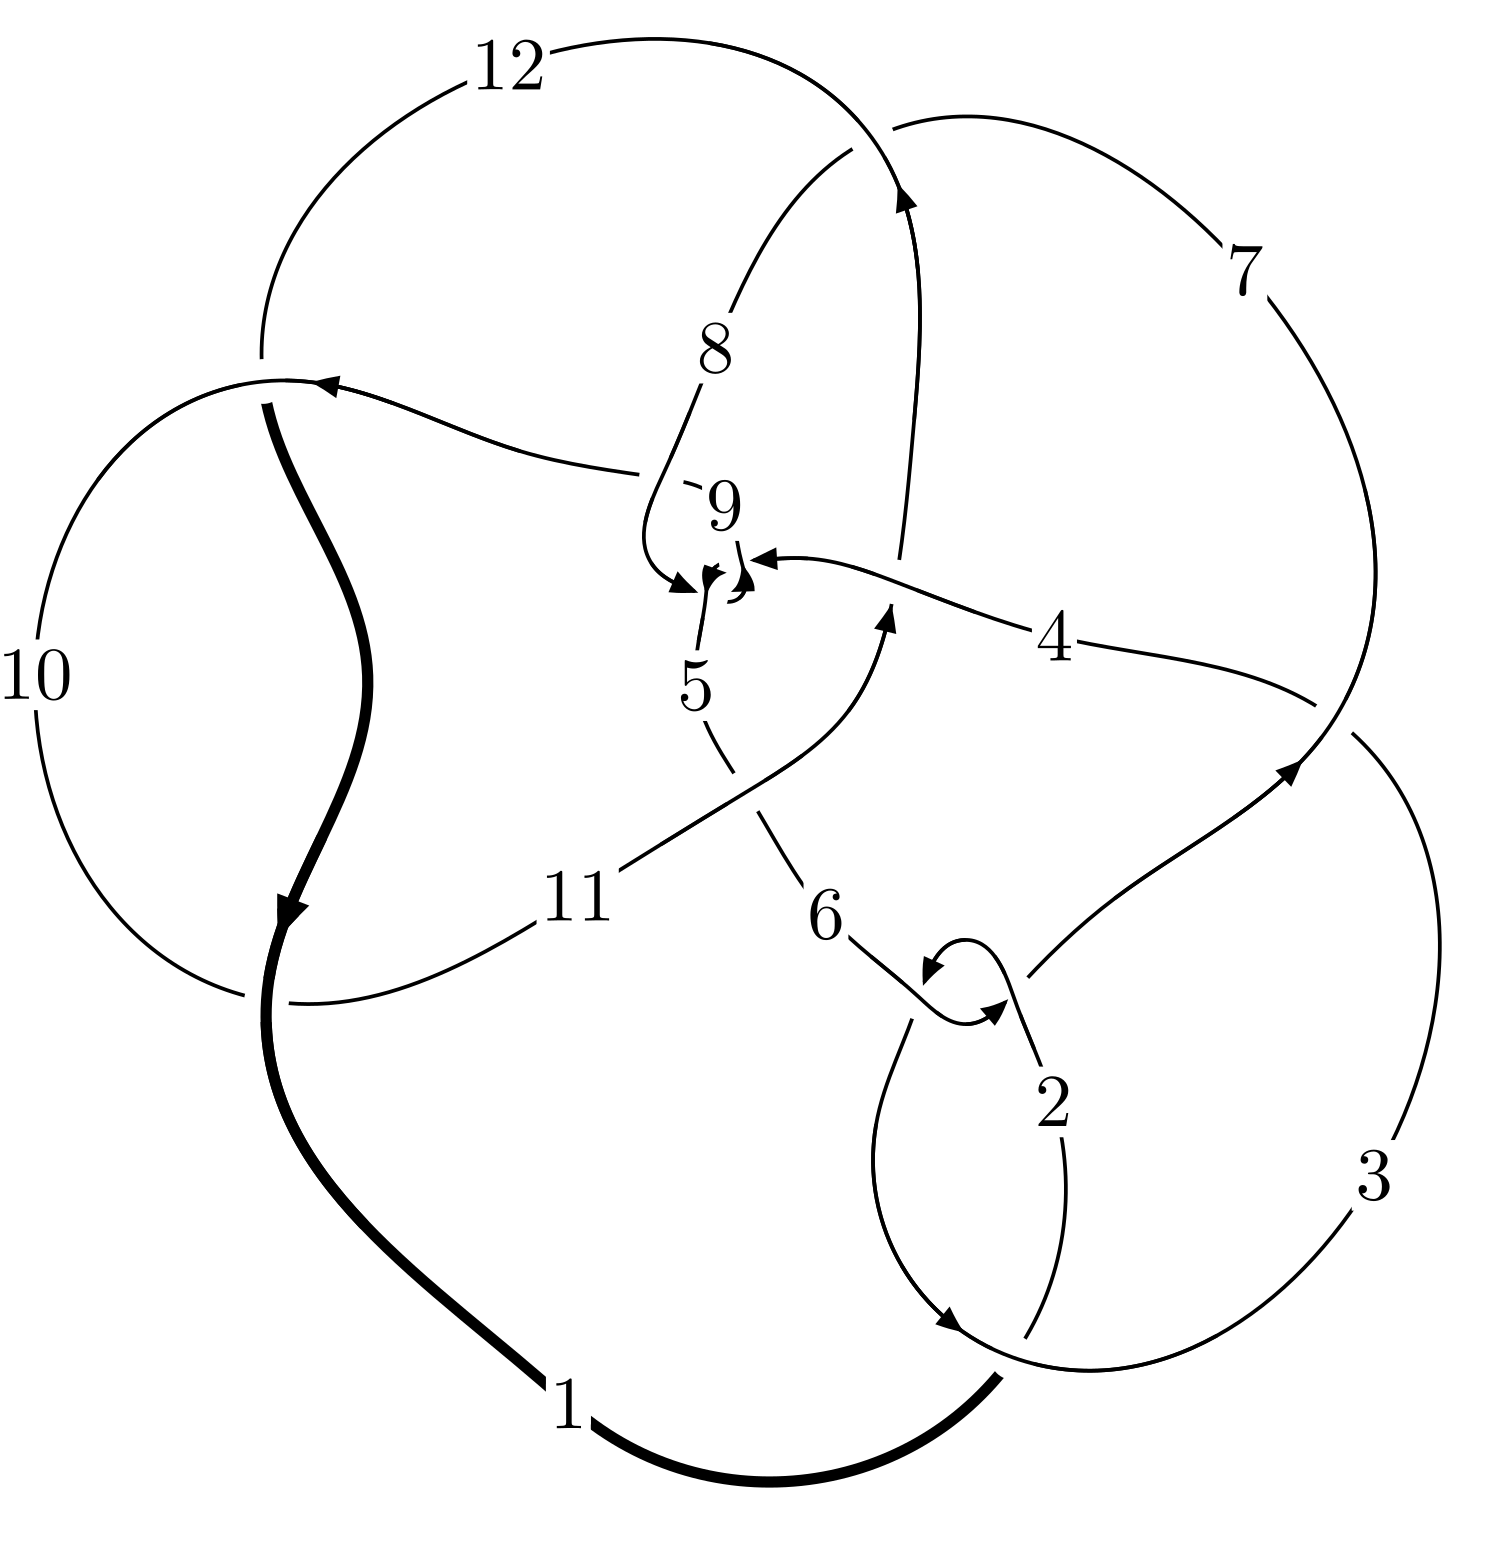
\includegraphics[width=112pt]{../../../GIT/diagram.site/Diagrams/png/1025_12a_0224.png}\\
\ \ \ A knot diagram\footnotemark}&
\allowdisplaybreaks
\textbf{Linearized knot diagam} \\
\cline{2-2}
 &
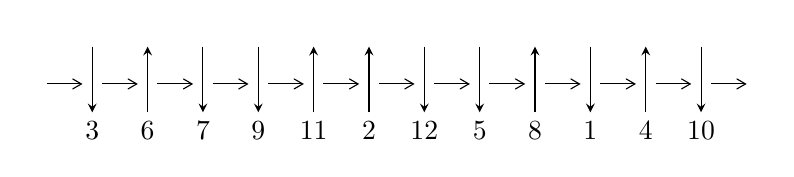
\begin{tikzpicture}[x=20pt, y=17pt]
	% nodes
	\node (C0) at (0, 0) {};
	\node (C1) at (1, 0) {};
	\node (C1U) at (1, +1) {};
	\node (C1D) at (1, -1) {3};

	\node (C2) at (2, 0) {};
	\node (C2U) at (2, +1) {};
	\node (C2D) at (2, -1) {6};

	\node (C3) at (3, 0) {};
	\node (C3U) at (3, +1) {};
	\node (C3D) at (3, -1) {7};

	\node (C4) at (4, 0) {};
	\node (C4U) at (4, +1) {};
	\node (C4D) at (4, -1) {9};

	\node (C5) at (5, 0) {};
	\node (C5U) at (5, +1) {};
	\node (C5D) at (5, -1) {11};

	\node (C6) at (6, 0) {};
	\node (C6U) at (6, +1) {};
	\node (C6D) at (6, -1) {2};

	\node (C7) at (7, 0) {};
	\node (C7U) at (7, +1) {};
	\node (C7D) at (7, -1) {12};

	\node (C8) at (8, 0) {};
	\node (C8U) at (8, +1) {};
	\node (C8D) at (8, -1) {5};

	\node (C9) at (9, 0) {};
	\node (C9U) at (9, +1) {};
	\node (C9D) at (9, -1) {8};

	\node (C10) at (10, 0) {};
	\node (C10U) at (10, +1) {};
	\node (C10D) at (10, -1) {1};

	\node (C11) at (11, 0) {};
	\node (C11U) at (11, +1) {};
	\node (C11D) at (11, -1) {4};

	\node (C12) at (12, 0) {};
	\node (C12U) at (12, +1) {};
	\node (C12D) at (12, -1) {10};
	\node (C13) at (13, 0) {};

	% arrows
	\draw[->,>={angle 60}]
	(C0) edge (C1) (C1) edge (C2) (C2) edge (C3) (C3) edge (C4) (C4) edge (C5) (C5) edge (C6) (C6) edge (C7) (C7) edge (C8) (C8) edge (C9) (C9) edge (C10) (C10) edge (C11) (C11) edge (C12) (C12) edge (C13) ;	\draw[->,>=stealth]
	(C1U) edge (C1D) (C2D) edge (C2U) (C3U) edge (C3D) (C4U) edge (C4D) (C5D) edge (C5U) (C6D) edge (C6U) (C7U) edge (C7D) (C8U) edge (C8D) (C9D) edge (C9U) (C10U) edge (C10D) (C11D) edge (C11U) (C12U) edge (C12D) ;
	\end{tikzpicture} \\
\hhline{~~} \\& 
\textbf{Solving Sequence} \\ \cline{2-2} 
 &
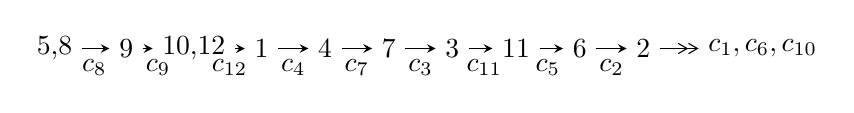
\begin{tikzpicture}[x=23pt, y=7pt]
	% node
	\node (A0) at (-1/8, 0) {5,8};
	\node (A1) at (1, 0) {9};
	\node (A2) at (33/16, 0) {10,12};
	\node (A3) at (25/8, 0) {1};
	\node (A4) at (33/8, 0) {4};
	\node (A5) at (41/8, 0) {7};
	\node (A6) at (49/8, 0) {3};
	\node (A7) at (57/8, 0) {11};
	\node (A8) at (65/8, 0) {6};
	\node (A9) at (73/8, 0) {2};
	\node (C1) at (1/2, -1) {$c_{8}$};
	\node (C2) at (3/2, -1) {$c_{9}$};
	\node (C3) at (21/8, -1) {$c_{12}$};
	\node (C4) at (29/8, -1) {$c_{4}$};
	\node (C5) at (37/8, -1) {$c_{7}$};
	\node (C6) at (45/8, -1) {$c_{3}$};
	\node (C7) at (53/8, -1) {$c_{11}$};
	\node (C8) at (61/8, -1) {$c_{5}$};
	\node (C9) at (69/8, -1) {$c_{2}$};
	\node (A10) at (11, 0) {$c_{1},c_{6},c_{10}$};

	% edge
	\draw[->,>=stealth]	
	(A0) edge (A1) (A1) edge (A2) (A2) edge (A3) (A3) edge (A4) (A4) edge (A5) (A5) edge (A6) (A6) edge (A7) (A7) edge (A8) (A8) edge (A9) ;
	\draw[->>,>={angle 60}]	
	(A9) edge (A10);
\end{tikzpicture} \\ 

\end{tabular} \\

\footnotetext{
The image of knot diagram is generated by the software ``\textbf{Draw programme}" developed by Andrew Bartholomew(\url{http://www.layer8.co.uk/maths/draw/index.htm\#Running-draw}), where we modified some parts for our purpose(\url{https://github.com/CATsTAILs/LinksPainter}).
}\phantom \\ \newline 
\centering \textbf{Ideals for irreducible components\footnotemark of $X_{\text{par}}$} 
 
\begin{align*}
I^u_{1}&=\langle 
5.54139\times10^{211} u^{118}-1.77953\times10^{212} u^{117}+\cdots+1.16640\times10^{212} b+2.45569\times10^{210},\\
\phantom{I^u_{1}}&\phantom{= \langle  }1.48602\times10^{212} u^{118}-2.52384\times10^{212} u^{117}+\cdots+1.16640\times10^{212} a-2.66943\times10^{212},\;u^{119}-2 u^{118}+\cdots+4 u-1\rangle \\
I^u_{2}&=\langle 
-2 u^3-10 u^2+13 b-7 u-19,\;-7 u^3-9 u^2+13 a-18 u-21,\;u^4+u^3+3 u^2+2 u+1\rangle \\
\\
\end{align*}
\raggedright * 2 irreducible components of $\dim_{\mathbb{C}}=0$, with total 123 representations.\\
\footnotetext{All coefficients of polynomials are rational numbers. But the coefficients are sometimes approximated in decimal forms when there is not enough margin.}
\newpage
\renewcommand{\arraystretch}{1}
\centering \section*{I. $I^u_{1}= \langle 5.54\times10^{211} u^{118}-1.78\times10^{212} u^{117}+\cdots+1.17\times10^{212} b+2.46\times10^{210},\;1.49\times10^{212} u^{118}-2.52\times10^{212} u^{117}+\cdots+1.17\times10^{212} a-2.67\times10^{212},\;u^{119}-2 u^{118}+\cdots+4 u-1 \rangle$}
\flushleft \textbf{(i) Arc colorings}\\
\begin{tabular}{m{7pt} m{180pt} m{7pt} m{180pt} }
\flushright $a_{5}=$&$\begin{pmatrix}0\\u\end{pmatrix}$ \\
\flushright $a_{8}=$&$\begin{pmatrix}1\\0\end{pmatrix}$ \\
\flushright $a_{9}=$&$\begin{pmatrix}1\\u^2\end{pmatrix}$ \\
\flushright $a_{10}=$&$\begin{pmatrix}u^2+1\\u^2\end{pmatrix}$ \\
\flushright $a_{12}=$&$\begin{pmatrix}-1.27402 u^{118}+2.16379 u^{117}+\cdots+3.90194 u+2.28861\\-0.475087 u^{118}+1.52566 u^{117}+\cdots+3.68582 u-0.0210536\end{pmatrix}$ \\
\flushright $a_{1}=$&$\begin{pmatrix}-1.05425 u^{118}+1.73753 u^{117}+\cdots+2.83349 u+1.51971\\-0.511788 u^{118}+1.44255 u^{117}+\cdots+3.26316 u+0.148729\end{pmatrix}$ \\
\flushright $a_{4}=$&$\begin{pmatrix}u\\u^3+u\end{pmatrix}$ \\
\flushright $a_{7}=$&$\begin{pmatrix}5.78938 u^{118}-9.05492 u^{117}+\cdots-16.0766 u+1.50354\\2.96804 u^{118}-7.67244 u^{117}+\cdots-18.0668 u+4.40843\end{pmatrix}$ \\
\flushright $a_{3}=$&$\begin{pmatrix}0.800386 u^{118}-0.654146 u^{117}+\cdots-2.68625 u+1.50085\\1.52874 u^{118}-2.03781 u^{117}+\cdots-4.20547 u+1.56993\end{pmatrix}$ \\
\flushright $a_{11}=$&$\begin{pmatrix}-1.24679 u^{118}+2.17866 u^{117}+\cdots+4.01135 u+2.22723\\-0.409852 u^{118}+1.43273 u^{117}+\cdots+3.54515 u-0.0131086\end{pmatrix}$ \\
\flushright $a_{6}=$&$\begin{pmatrix}-4.27793 u^{118}+6.86729 u^{117}+\cdots+26.0602 u-4.12891\\-2.27112 u^{118}+6.74915 u^{117}+\cdots+21.1757 u-5.07591\end{pmatrix}$ \\
\flushright $a_{2}=$&$\begin{pmatrix}0.0164683 u^{118}+0.631381 u^{117}+\cdots+3.64517 u+0.716005\\-0.625567 u^{118}+1.59469 u^{117}+\cdots+0.143061 u+0.960630\end{pmatrix}$\\&\end{tabular}
\flushleft \textbf{(ii) Obstruction class $= -1$}\\~\\
\flushleft \textbf{(iii) Cusp Shapes $= 8.20464 u^{118}-9.79230 u^{117}+\cdots-12.0561 u-5.30921$}\\~\\
\newpage\renewcommand{\arraystretch}{1}
\flushleft \textbf{(iv) u-Polynomials at the component}\newline \\
\begin{tabular}{m{50pt}|m{274pt}}
Crossings & \hspace{64pt}u-Polynomials at each crossing \\
\hline $$\begin{aligned}c_{1}\end{aligned}$$&$\begin{aligned}
&u^{119}+60 u^{118}+\cdots-4 u-1
\end{aligned}$\\
\hline $$\begin{aligned}c_{2},c_{6}\end{aligned}$$&$\begin{aligned}
&u^{119}-2 u^{118}+\cdots+2 u-1
\end{aligned}$\\
\hline $$\begin{aligned}c_{3}\end{aligned}$$&$\begin{aligned}
&u^{119}+2 u^{118}+\cdots-391360 u-162248
\end{aligned}$\\
\hline $$\begin{aligned}c_{4},c_{8}\end{aligned}$$&$\begin{aligned}
&u^{119}+2 u^{118}+\cdots+4 u+1
\end{aligned}$\\
\hline $$\begin{aligned}c_{5}\end{aligned}$$&$\begin{aligned}
&13(13 u^{119}+45 u^{118}+\cdots-9.53716\times10^{7} u+8.13301\times10^{7})
\end{aligned}$\\
\hline $$\begin{aligned}c_{7}\end{aligned}$$&$\begin{aligned}
&13(13 u^{119}+72 u^{118}+\cdots+3.83586\times10^{7} u+1.67631\times10^{7})
\end{aligned}$\\
\hline $$\begin{aligned}c_{9}\end{aligned}$$&$\begin{aligned}
&u^{119}-48 u^{118}+\cdots-4 u+1
\end{aligned}$\\
\hline $$\begin{aligned}c_{10},c_{12}\end{aligned}$$&$\begin{aligned}
&u^{119}-5 u^{118}+\cdots+4638 u+169
\end{aligned}$\\
\hline $$\begin{aligned}c_{11}\end{aligned}$$&$\begin{aligned}
&u^{119}-5 u^{118}+\cdots-3016 u+2704
\end{aligned}$\\
\hline
\end{tabular}\\~\\
\newpage\renewcommand{\arraystretch}{1}
\flushleft \textbf{(v) Riley Polynomials at the component}\newline \\
\begin{tabular}{m{50pt}|m{274pt}}
Crossings & \hspace{64pt}Riley Polynomials at each crossing \\
\hline $$\begin{aligned}c_{1}\end{aligned}$$&$\begin{aligned}
&y^{119}+120 y^{117}+\cdots+8 y-1
\end{aligned}$\\
\hline $$\begin{aligned}c_{2},c_{6}\end{aligned}$$&$\begin{aligned}
&y^{119}+60 y^{118}+\cdots-4 y-1
\end{aligned}$\\
\hline $$\begin{aligned}c_{3}\end{aligned}$$&$\begin{aligned}
&y^{119}-60 y^{118}+\cdots-1006938781552 y-26324413504
\end{aligned}$\\
\hline $$\begin{aligned}c_{4},c_{8}\end{aligned}$$&$\begin{aligned}
&y^{119}+48 y^{118}+\cdots-4 y-1
\end{aligned}$\\
\hline $$\begin{aligned}c_{5}\end{aligned}$$&$\begin{aligned}
&169(169 y^{119}+20465 y^{118}+\cdots-3.94300\times10^{17} y-6.61458\times10^{15})
\end{aligned}$\\
\hline $$\begin{aligned}c_{7}\end{aligned}$$&$\begin{aligned}
&169\\
&\cdot(169 y^{119}+1134 y^{118}+\cdots+560619390409464 y-281003063817316)
\end{aligned}$\\
\hline $$\begin{aligned}c_{9}\end{aligned}$$&$\begin{aligned}
&y^{119}+48 y^{118}+\cdots-112 y-1
\end{aligned}$\\
\hline $$\begin{aligned}c_{10},c_{12}\end{aligned}$$&$\begin{aligned}
&y^{119}-93 y^{118}+\cdots+1876286 y-28561
\end{aligned}$\\
\hline $$\begin{aligned}c_{11}\end{aligned}$$&$\begin{aligned}
&y^{119}+27 y^{118}+\cdots-531184576 y-7311616
\end{aligned}$\\
\hline
\end{tabular}\\~\\
\newpage\flushleft \textbf{(vi) Complex Volumes and Cusp Shapes}
$$\begin{array}{c|c|c}  
\text{Solutions to }I^u_{1}& \I (\text{vol} + \sqrt{-1}CS) & \text{Cusp shape}\\
 \hline 
\begin{aligned}
u &= \phantom{-}0.539418 + 0.840998 I \\
a &= -1.41285 - 3.92453 I \\
b &= \phantom{-}2.86930 - 3.88516 I\end{aligned}
 & -1.82418 - 1.97603 I & \phantom{-0.000000 } 0 \\ \hline\begin{aligned}
u &= \phantom{-}0.539418 - 0.840998 I \\
a &= -1.41285 + 3.92453 I \\
b &= \phantom{-}2.86930 + 3.88516 I\end{aligned}
 & -1.82418 + 1.97603 I & \phantom{-0.000000 } 0 \\ \hline\begin{aligned}
u &= \phantom{-}0.046971 + 1.018560 I \\
a &= -0.028457 - 0.767848 I \\
b &= -0.679310 + 1.026440 I\end{aligned}
 & \phantom{-}0.75162 + 6.45433 I & \phantom{-0.000000 } 0 \\ \hline\begin{aligned}
u &= \phantom{-}0.046971 - 1.018560 I \\
a &= -0.028457 + 0.767848 I \\
b &= -0.679310 - 1.026440 I\end{aligned}
 & \phantom{-}0.75162 - 6.45433 I & \phantom{-0.000000 } 0 \\ \hline\begin{aligned}
u &= -0.078413 + 1.020000 I \\
a &= \phantom{-}0.003241 + 0.649226 I \\
b &= -0.534367 - 0.951411 I\end{aligned}
 & \phantom{-}3.26046 - 1.73121 I & \phantom{-0.000000 } 0 \\ \hline\begin{aligned}
u &= -0.078413 - 1.020000 I \\
a &= \phantom{-}0.003241 - 0.649226 I \\
b &= -0.534367 + 0.951411 I\end{aligned}
 & \phantom{-}3.26046 + 1.73121 I & \phantom{-0.000000 } 0 \\ \hline\begin{aligned}
u &= -0.659946 + 0.783354 I \\
a &= \phantom{-}1.283510 - 0.311392 I \\
b &= \phantom{-}0.969241 + 0.277435 I\end{aligned}
 & -5.03562 + 0.41103 I & \phantom{-0.000000 } 0 \\ \hline\begin{aligned}
u &= -0.659946 - 0.783354 I \\
a &= \phantom{-}1.283510 + 0.311392 I \\
b &= \phantom{-}0.969241 - 0.277435 I\end{aligned}
 & -5.03562 - 0.41103 I & \phantom{-0.000000 } 0 \\ \hline\begin{aligned}
u &= \phantom{-}0.673685 + 0.775129 I \\
a &= \phantom{-}1.55336 + 0.38532 I \\
b &= \phantom{-}1.037470 - 0.181769 I\end{aligned}
 & -8.13975 + 3.86403 I & \phantom{-0.000000 } 0 \\ \hline\begin{aligned}
u &= \phantom{-}0.673685 - 0.775129 I \\
a &= \phantom{-}1.55336 - 0.38532 I \\
b &= \phantom{-}1.037470 + 0.181769 I\end{aligned}
 & -8.13975 - 3.86403 I & \phantom{-0.000000 } 0\\
 \hline 
 \end{array}$$\newpage$$\begin{array}{c|c|c}  
\text{Solutions to }I^u_{1}& \I (\text{vol} + \sqrt{-1}CS) & \text{Cusp shape}\\
 \hline 
\begin{aligned}
u &= \phantom{-}0.671736 + 0.796619 I \\
a &= \phantom{-}1.240250 + 0.644710 I \\
b &= \phantom{-}0.855354 - 0.170542 I\end{aligned}
 & -8.40527 - 4.37677 I & \phantom{-0.000000 } 0 \\ \hline\begin{aligned}
u &= \phantom{-}0.671736 - 0.796619 I \\
a &= \phantom{-}1.240250 - 0.644710 I \\
b &= \phantom{-}0.855354 + 0.170542 I\end{aligned}
 & -8.40527 + 4.37677 I & \phantom{-0.000000 } 0 \\ \hline\begin{aligned}
u &= -0.608259 + 0.726692 I \\
a &= \phantom{-}1.55701 + 0.53379 I \\
b &= \phantom{-}1.251790 + 0.275028 I\end{aligned}
 & -3.42582 - 0.69701 I & \phantom{-0.000000 } 0 \\ \hline\begin{aligned}
u &= -0.608259 - 0.726692 I \\
a &= \phantom{-}1.55701 - 0.53379 I \\
b &= \phantom{-}1.251790 - 0.275028 I\end{aligned}
 & -3.42582 + 0.69701 I & \phantom{-0.000000 } 0 \\ \hline\begin{aligned}
u &= \phantom{-}0.559945 + 0.891958 I \\
a &= -2.93671 + 0.94418 I \\
b &= -1.96748 - 2.48153 I\end{aligned}
 & -1.62898 - 2.41378 I & \phantom{-0.000000 } 0 \\ \hline\begin{aligned}
u &= \phantom{-}0.559945 - 0.891958 I \\
a &= -2.93671 - 0.94418 I \\
b &= -1.96748 + 2.48153 I\end{aligned}
 & -1.62898 + 2.41378 I & \phantom{-0.000000 } 0 \\ \hline\begin{aligned}
u &= -0.633152 + 0.845568 I \\
a &= -0.148666 - 0.555779 I \\
b &= \phantom{-}0.252806 + 0.751615 I\end{aligned}
 & -4.67693 + 2.47706 I & \phantom{-0.000000 } 0 \\ \hline\begin{aligned}
u &= -0.633152 - 0.845568 I \\
a &= -0.148666 + 0.555779 I \\
b &= \phantom{-}0.252806 - 0.751615 I\end{aligned}
 & -4.67693 - 2.47706 I & \phantom{-0.000000 } 0 \\ \hline\begin{aligned}
u &= -0.446454 + 0.824660 I \\
a &= \phantom{-}5.44391 - 1.11040 I \\
b &= \phantom{-}1.60652 - 4.51876 I\end{aligned}
 & -4.00299 - 1.55704 I & \phantom{-0.000000 } 0 \\ \hline\begin{aligned}
u &= -0.446454 - 0.824660 I \\
a &= \phantom{-}5.44391 + 1.11040 I \\
b &= \phantom{-}1.60652 + 4.51876 I\end{aligned}
 & -4.00299 + 1.55704 I & \phantom{-0.000000 } 0\\
 \hline 
 \end{array}$$\newpage$$\begin{array}{c|c|c}  
\text{Solutions to }I^u_{1}& \I (\text{vol} + \sqrt{-1}CS) & \text{Cusp shape}\\
 \hline 
\begin{aligned}
u &= \phantom{-}0.069950 + 0.934961 I \\
a &= \phantom{-}0.312469 - 0.726574 I \\
b &= -0.673000 + 0.632241 I\end{aligned}
 & -0.626086 - 1.186890 I & \phantom{-0.000000 } 0 \\ \hline\begin{aligned}
u &= \phantom{-}0.069950 - 0.934961 I \\
a &= \phantom{-}0.312469 + 0.726574 I \\
b &= -0.673000 - 0.632241 I\end{aligned}
 & -0.626086 + 1.186890 I & \phantom{-0.000000 } 0 \\ \hline\begin{aligned}
u &= \phantom{-}0.917495 + 0.542434 I \\
a &= -1.25859 + 0.96564 I \\
b &= -1.49694 + 0.80766 I\end{aligned}
 & -9.6630 + 13.1992 I & \phantom{-0.000000 } 0 \\ \hline\begin{aligned}
u &= \phantom{-}0.917495 - 0.542434 I \\
a &= -1.25859 - 0.96564 I \\
b &= -1.49694 - 0.80766 I\end{aligned}
 & -9.6630 - 13.1992 I & \phantom{-0.000000 } 0 \\ \hline\begin{aligned}
u &= -0.922448 + 0.546566 I \\
a &= -1.17166 - 0.90511 I \\
b &= -1.42673 - 0.77297 I\end{aligned}
 & -6.80262 - 7.99479 I & \phantom{-0.000000 } 0 \\ \hline\begin{aligned}
u &= -0.922448 - 0.546566 I \\
a &= -1.17166 + 0.90511 I \\
b &= -1.42673 + 0.77297 I\end{aligned}
 & -6.80262 + 7.99479 I & \phantom{-0.000000 } 0 \\ \hline\begin{aligned}
u &= \phantom{-}0.930348 + 0.539182 I \\
a &= -1.22943 + 0.74279 I \\
b &= -1.45164 + 0.64689 I\end{aligned}
 & -11.52010 + 4.26179 I & \phantom{-0.000000 } 0 \\ \hline\begin{aligned}
u &= \phantom{-}0.930348 - 0.539182 I \\
a &= -1.22943 - 0.74279 I \\
b &= -1.45164 - 0.64689 I\end{aligned}
 & -11.52010 - 4.26179 I & \phantom{-0.000000 } 0 \\ \hline\begin{aligned}
u &= -0.974458 + 0.464052 I \\
a &= -0.767249 + 0.225407 I \\
b &= -1.016070 + 0.066000 I\end{aligned}
 & -9.08388 + 8.22471 I & \phantom{-0.000000 } 0 \\ \hline\begin{aligned}
u &= -0.974458 - 0.464052 I \\
a &= -0.767249 - 0.225407 I \\
b &= -1.016070 - 0.066000 I\end{aligned}
 & -9.08388 - 8.22471 I & \phantom{-0.000000 } 0\\
 \hline 
 \end{array}$$\newpage$$\begin{array}{c|c|c}  
\text{Solutions to }I^u_{1}& \I (\text{vol} + \sqrt{-1}CS) & \text{Cusp shape}\\
 \hline 
\begin{aligned}
u &= -0.550074 + 0.933763 I \\
a &= \phantom{-}0.14546 - 1.56145 I \\
b &= -1.17975 - 0.97383 I\end{aligned}
 & -2.72220 - 1.73214 I & \phantom{-0.000000 } 0 \\ \hline\begin{aligned}
u &= -0.550074 - 0.933763 I \\
a &= \phantom{-}0.14546 + 1.56145 I \\
b &= -1.17975 + 0.97383 I\end{aligned}
 & -2.72220 + 1.73214 I & \phantom{-0.000000 } 0 \\ \hline\begin{aligned}
u &= -0.551834 + 0.943079 I \\
a &= -0.79925 - 2.16152 I \\
b &= -2.09153 - 0.35978 I\end{aligned}
 & -3.33941 + 5.68580 I & \phantom{-0.000000 } 0 \\ \hline\begin{aligned}
u &= -0.551834 - 0.943079 I \\
a &= -0.79925 + 2.16152 I \\
b &= -2.09153 + 0.35978 I\end{aligned}
 & -3.33941 - 5.68580 I & \phantom{-0.000000 } 0 \\ \hline\begin{aligned}
u &= \phantom{-}0.659514 + 0.622337 I \\
a &= \phantom{-}1.72648 - 0.86511 I \\
b &= \phantom{-}0.923703 - 0.477948 I\end{aligned}
 & -5.12870 - 0.71737 I & \phantom{-0.000000 } 0 \\ \hline\begin{aligned}
u &= \phantom{-}0.659514 - 0.622337 I \\
a &= \phantom{-}1.72648 + 0.86511 I \\
b &= \phantom{-}0.923703 + 0.477948 I\end{aligned}
 & -5.12870 + 0.71737 I & \phantom{-0.000000 } 0 \\ \hline\begin{aligned}
u &= \phantom{-}0.533310 + 0.955795 I \\
a &= -0.355768 + 1.171140 I \\
b &= -1.059370 + 0.421671 I\end{aligned}
 & -0.16207 - 2.47699 I & \phantom{-0.000000 } 0 \\ \hline\begin{aligned}
u &= \phantom{-}0.533310 - 0.955795 I \\
a &= -0.355768 - 1.171140 I \\
b &= -1.059370 - 0.421671 I\end{aligned}
 & -0.16207 + 2.47699 I & \phantom{-0.000000 } 0 \\ \hline\begin{aligned}
u &= -0.973549 + 0.502306 I \\
a &= -0.925732 - 0.061551 I \\
b &= -1.155010 - 0.152766 I\end{aligned}
 & -11.15970 - 0.90036 I & \phantom{-0.000000 } 0 \\ \hline\begin{aligned}
u &= -0.973549 - 0.502306 I \\
a &= -0.925732 + 0.061551 I \\
b &= -1.155010 + 0.152766 I\end{aligned}
 & -11.15970 + 0.90036 I & \phantom{-0.000000 } 0\\
 \hline 
 \end{array}$$\newpage$$\begin{array}{c|c|c}  
\text{Solutions to }I^u_{1}& \I (\text{vol} + \sqrt{-1}CS) & \text{Cusp shape}\\
 \hline 
\begin{aligned}
u &= -0.130607 + 1.092120 I \\
a &= -0.134163 + 0.411423 I \\
b &= -0.144643 - 0.954492 I\end{aligned}
 & \phantom{-}4.94213 - 0.22183 I & \phantom{-0.000000 } 0 \\ \hline\begin{aligned}
u &= -0.130607 - 1.092120 I \\
a &= -0.134163 - 0.411423 I \\
b &= -0.144643 + 0.954492 I\end{aligned}
 & \phantom{-}4.94213 + 0.22183 I & \phantom{-0.000000 } 0 \\ \hline\begin{aligned}
u &= \phantom{-}0.682031 + 0.587060 I \\
a &= \phantom{-}1.59450 - 1.08081 I \\
b &= \phantom{-}0.774323 - 0.632613 I\end{aligned}
 & -4.10775 + 7.30854 I & \phantom{-0.000000 } 0 \\ \hline\begin{aligned}
u &= \phantom{-}0.682031 - 0.587060 I \\
a &= \phantom{-}1.59450 + 1.08081 I \\
b &= \phantom{-}0.774323 + 0.632613 I\end{aligned}
 & -4.10775 - 7.30854 I & \phantom{-0.000000 } 0 \\ \hline\begin{aligned}
u &= \phantom{-}0.994202 + 0.476764 I \\
a &= -0.713312 - 0.073664 I \\
b &= -0.978129 + 0.056427 I\end{aligned}
 & -6.20252 - 2.86568 I & \phantom{-0.000000 } 0 \\ \hline\begin{aligned}
u &= \phantom{-}0.994202 - 0.476764 I \\
a &= -0.713312 + 0.073664 I \\
b &= -0.978129 - 0.056427 I\end{aligned}
 & -6.20252 + 2.86568 I & \phantom{-0.000000 } 0 \\ \hline\begin{aligned}
u &= -0.948881 + 0.578795 I \\
a &= -0.737186 - 0.750921 I \\
b &= -1.083840 - 0.714353 I\end{aligned}
 & -3.26565 - 5.72258 I & \phantom{-0.000000 } 0 \\ \hline\begin{aligned}
u &= -0.948881 - 0.578795 I \\
a &= -0.737186 + 0.750921 I \\
b &= -1.083840 + 0.714353 I\end{aligned}
 & -3.26565 + 5.72258 I & \phantom{-0.000000 } 0 \\ \hline\begin{aligned}
u &= \phantom{-}0.663407 + 0.892584 I \\
a &= -0.70152 + 1.69641 I \\
b &= -0.523674 - 0.243591 I\end{aligned}
 & -8.11332 - 0.79069 I & \phantom{-0.000000 } 0 \\ \hline\begin{aligned}
u &= \phantom{-}0.663407 - 0.892584 I \\
a &= -0.70152 - 1.69641 I \\
b &= -0.523674 + 0.243591 I\end{aligned}
 & -8.11332 + 0.79069 I & \phantom{-0.000000 } 0\\
 \hline 
 \end{array}$$\newpage$$\begin{array}{c|c|c}  
\text{Solutions to }I^u_{1}& \I (\text{vol} + \sqrt{-1}CS) & \text{Cusp shape}\\
 \hline 
\begin{aligned}
u &= -0.653196 + 0.902505 I \\
a &= -0.96221 - 1.58214 I \\
b &= -0.673782 + 0.386392 I\end{aligned}
 & -4.67219 + 4.69161 I & \phantom{-0.000000 } 0 \\ \hline\begin{aligned}
u &= -0.653196 - 0.902505 I \\
a &= -0.96221 + 1.58214 I \\
b &= -0.673782 - 0.386392 I\end{aligned}
 & -4.67219 - 4.69161 I & \phantom{-0.000000 } 0 \\ \hline\begin{aligned}
u &= -0.613693 + 0.933505 I \\
a &= -1.46824 - 1.31363 I \\
b &= -1.142650 + 0.651183 I\end{aligned}
 & -2.79223 + 5.53654 I & \phantom{-0.000000 } 0 \\ \hline\begin{aligned}
u &= -0.613693 - 0.933505 I \\
a &= -1.46824 + 1.31363 I \\
b &= -1.142650 - 0.651183 I\end{aligned}
 & -2.79223 - 5.53654 I & \phantom{-0.000000 } 0 \\ \hline\begin{aligned}
u &= -0.658134 + 0.582283 I \\
a &= \phantom{-}1.52930 + 0.95183 I \\
b &= \phantom{-}0.732852 + 0.515230 I\end{aligned}
 & -1.37744 - 2.68961 I & \phantom{-0.000000 } 0 \\ \hline\begin{aligned}
u &= -0.658134 - 0.582283 I \\
a &= \phantom{-}1.52930 - 0.95183 I \\
b &= \phantom{-}0.732852 - 0.515230 I\end{aligned}
 & -1.37744 + 2.68961 I & \phantom{-0.000000 } 0 \\ \hline\begin{aligned}
u &= \phantom{-}0.662513 + 0.909459 I \\
a &= -1.03375 + 1.78951 I \\
b &= -0.765897 - 0.257992 I\end{aligned}
 & -7.73252 - 9.03670 I & \phantom{-0.000000 } 0 \\ \hline\begin{aligned}
u &= \phantom{-}0.662513 - 0.909459 I \\
a &= -1.03375 - 1.78951 I \\
b &= -0.765897 + 0.257992 I\end{aligned}
 & -7.73252 + 9.03670 I & \phantom{-0.000000 } 0 \\ \hline\begin{aligned}
u &= \phantom{-}0.987963 + 0.581470 I \\
a &= -0.596782 + 0.532091 I \\
b &= -0.940516 + 0.566068 I\end{aligned}
 & -2.98815 + 0.27290 I & \phantom{-0.000000 } 0 \\ \hline\begin{aligned}
u &= \phantom{-}0.987963 - 0.581470 I \\
a &= -0.596782 - 0.532091 I \\
b &= -0.940516 - 0.566068 I\end{aligned}
 & -2.98815 - 0.27290 I & \phantom{-0.000000 } 0\\
 \hline 
 \end{array}$$\newpage$$\begin{array}{c|c|c}  
\text{Solutions to }I^u_{1}& \I (\text{vol} + \sqrt{-1}CS) & \text{Cusp shape}\\
 \hline 
\begin{aligned}
u &= -0.351471 + 0.773470 I \\
a &= \phantom{-}2.58714 - 1.56388 I \\
b &= -0.30248 - 2.06274 I\end{aligned}
 & -3.60723 + 5.96757 I & \phantom{-0.000000 } 0 \\ \hline\begin{aligned}
u &= -0.351471 - 0.773470 I \\
a &= \phantom{-}2.58714 + 1.56388 I \\
b &= -0.30248 + 2.06274 I\end{aligned}
 & -3.60723 - 5.96757 I & \phantom{-0.000000 } 0 \\ \hline\begin{aligned}
u &= \phantom{-}0.153792 + 1.146450 I \\
a &= -0.197319 - 0.303202 I \\
b &= \phantom{-}0.084898 + 0.871312 I\end{aligned}
 & \phantom{-}4.36424 - 4.50432 I & \phantom{-0.000000 } 0 \\ \hline\begin{aligned}
u &= \phantom{-}0.153792 - 1.146450 I \\
a &= -0.197319 + 0.303202 I \\
b &= \phantom{-}0.084898 - 0.871312 I\end{aligned}
 & \phantom{-}4.36424 + 4.50432 I & \phantom{-0.000000 } 0 \\ \hline\begin{aligned}
u &= \phantom{-}0.428182 + 0.707297 I \\
a &= \phantom{-}2.25893 + 0.55909 I \\
b &= \phantom{-}0.55178 + 1.36307 I\end{aligned}
 & -1.00838 - 1.74591 I & \phantom{-0.000000 } 0 \\ \hline\begin{aligned}
u &= \phantom{-}0.428182 - 0.707297 I \\
a &= \phantom{-}2.25893 - 0.55909 I \\
b &= \phantom{-}0.55178 - 1.36307 I\end{aligned}
 & -1.00838 + 1.74591 I & \phantom{-0.000000 } 0 \\ \hline\begin{aligned}
u &= \phantom{-}0.364581 + 0.735982 I \\
a &= \phantom{-}0.980469 + 0.160216 I \\
b &= -0.057859 + 0.579273 I\end{aligned}
 & \phantom{-}0.01215 - 1.54922 I & \phantom{-0.000000 } 0 \\ \hline\begin{aligned}
u &= \phantom{-}0.364581 - 0.735982 I \\
a &= \phantom{-}0.980469 - 0.160216 I \\
b &= -0.057859 - 0.579273 I\end{aligned}
 & \phantom{-}0.01215 + 1.54922 I & \phantom{-0.000000 } 0 \\ \hline\begin{aligned}
u &= \phantom{-}0.630700 + 0.997407 I \\
a &= -1.87823 + 0.89275 I \\
b &= -1.085260 - 0.620294 I\end{aligned}
 & -4.02362 - 4.33336 I & \phantom{-0.000000 } 0 \\ \hline\begin{aligned}
u &= \phantom{-}0.630700 - 0.997407 I \\
a &= -1.87823 - 0.89275 I \\
b &= -1.085260 + 0.620294 I\end{aligned}
 & -4.02362 + 4.33336 I & \phantom{-0.000000 } 0\\
 \hline 
 \end{array}$$\newpage$$\begin{array}{c|c|c}  
\text{Solutions to }I^u_{1}& \I (\text{vol} + \sqrt{-1}CS) & \text{Cusp shape}\\
 \hline 
\begin{aligned}
u &= \phantom{-}0.570892 + 1.041270 I \\
a &= -1.090840 + 0.298866 I \\
b &= -0.607006 - 0.322725 I\end{aligned}
 & \phantom{-}1.77634 - 2.48623 I & \phantom{-0.000000 } 0 \\ \hline\begin{aligned}
u &= \phantom{-}0.570892 - 1.041270 I \\
a &= -1.090840 - 0.298866 I \\
b &= -0.607006 + 0.322725 I\end{aligned}
 & \phantom{-}1.77634 + 2.48623 I & \phantom{-0.000000 } 0 \\ \hline\begin{aligned}
u &= -0.626255 + 1.012710 I \\
a &= -1.85586 - 0.63971 I \\
b &= -0.977706 + 0.667269 I\end{aligned}
 & -0.12752 + 7.72535 I & \phantom{-0.000000 } 0 \\ \hline\begin{aligned}
u &= -0.626255 - 1.012710 I \\
a &= -1.85586 + 0.63971 I \\
b &= -0.977706 - 0.667269 I\end{aligned}
 & -0.12752 - 7.72535 I & \phantom{-0.000000 } 0 \\ \hline\begin{aligned}
u &= -0.599316 + 1.030510 I \\
a &= -1.45023 - 0.37860 I \\
b &= -0.747793 + 0.523187 I\end{aligned}
 & \phantom{-}1.99991 + 6.77961 I & \phantom{-0.000000 } 0 \\ \hline\begin{aligned}
u &= -0.599316 - 1.030510 I \\
a &= -1.45023 + 0.37860 I \\
b &= -0.747793 - 0.523187 I\end{aligned}
 & \phantom{-}1.99991 - 6.77961 I & \phantom{-0.000000 } 0 \\ \hline\begin{aligned}
u &= \phantom{-}0.635102 + 1.014540 I \\
a &= -2.01018 + 0.62700 I \\
b &= -1.012350 - 0.736958 I\end{aligned}
 & -2.86181 - 12.42930 I & \phantom{-0.000000 } 0 \\ \hline\begin{aligned}
u &= \phantom{-}0.635102 - 1.014540 I \\
a &= -2.01018 - 0.62700 I \\
b &= -1.012350 + 0.736958 I\end{aligned}
 & -2.86181 + 12.42930 I & \phantom{-0.000000 } 0 \\ \hline\begin{aligned}
u &= -0.608097 + 0.485373 I \\
a &= \phantom{-}1.122160 + 0.734555 I \\
b &= \phantom{-}0.347130 + 0.332291 I\end{aligned}
 & \phantom{-}0.49419 - 1.95496 I & \phantom{-0.000000 } 0 \\ \hline\begin{aligned}
u &= -0.608097 - 0.485373 I \\
a &= \phantom{-}1.122160 - 0.734555 I \\
b &= \phantom{-}0.347130 - 0.332291 I\end{aligned}
 & \phantom{-}0.49419 + 1.95496 I & \phantom{-0.000000 } 0\\
 \hline 
 \end{array}$$\newpage$$\begin{array}{c|c|c}  
\text{Solutions to }I^u_{1}& \I (\text{vol} + \sqrt{-1}CS) & \text{Cusp shape}\\
 \hline 
\begin{aligned}
u &= -0.071841 + 1.265180 I \\
a &= -0.355437 + 0.135357 I \\
b &= \phantom{-}0.886169 - 0.725281 I\end{aligned}
 & -2.70501 + 11.17610 I & \phantom{-0.000000 } 0 \\ \hline\begin{aligned}
u &= -0.071841 - 1.265180 I \\
a &= -0.355437 - 0.135357 I \\
b &= \phantom{-}0.886169 + 0.725281 I\end{aligned}
 & -2.70501 - 11.17610 I & \phantom{-0.000000 } 0 \\ \hline\begin{aligned}
u &= \phantom{-}0.087038 + 1.275070 I \\
a &= -0.327605 - 0.135550 I \\
b &= \phantom{-}0.780458 + 0.645595 I\end{aligned}
 & \phantom{-}0.26047 - 5.97490 I & \phantom{-0.000000 } 0 \\ \hline\begin{aligned}
u &= \phantom{-}0.087038 - 1.275070 I \\
a &= -0.327605 + 0.135550 I \\
b &= \phantom{-}0.780458 - 0.645595 I\end{aligned}
 & \phantom{-}0.26047 + 5.97490 I & \phantom{-0.000000 } 0 \\ \hline\begin{aligned}
u &= -0.067606 + 1.303270 I \\
a &= -0.321966 + 0.090369 I \\
b &= \phantom{-}0.870196 - 0.448726 I\end{aligned}
 & -4.44384 + 2.05586 I & \phantom{-0.000000 } 0 \\ \hline\begin{aligned}
u &= -0.067606 - 1.303270 I \\
a &= -0.321966 - 0.090369 I \\
b &= \phantom{-}0.870196 + 0.448726 I\end{aligned}
 & -4.44384 - 2.05586 I & \phantom{-0.000000 } 0 \\ \hline\begin{aligned}
u &= \phantom{-}0.701980 + 1.107930 I \\
a &= \phantom{-}1.65747 - 0.94084 I \\
b &= \phantom{-}1.55337 + 1.05580 I\end{aligned}
 & -7.9282 - 19.1536 I & \phantom{-0.000000 } 0 \\ \hline\begin{aligned}
u &= \phantom{-}0.701980 - 1.107930 I \\
a &= \phantom{-}1.65747 + 0.94084 I \\
b &= \phantom{-}1.55337 - 1.05580 I\end{aligned}
 & -7.9282 + 19.1536 I & \phantom{-0.000000 } 0 \\ \hline\begin{aligned}
u &= -0.430980 + 0.536340 I \\
a &= \phantom{-}2.05565 - 1.34242 I \\
b &= \phantom{-}0.327938 - 1.261390 I\end{aligned}
 & -3.62566 + 6.02987 I & -6.64015 - 6.08277 I \\ \hline\begin{aligned}
u &= -0.430980 - 0.536340 I \\
a &= \phantom{-}2.05565 + 1.34242 I \\
b &= \phantom{-}0.327938 + 1.261390 I\end{aligned}
 & -3.62566 - 6.02987 I & -6.64015 + 6.08277 I\\
 \hline 
 \end{array}$$\newpage$$\begin{array}{c|c|c}  
\text{Solutions to }I^u_{1}& \I (\text{vol} + \sqrt{-1}CS) & \text{Cusp shape}\\
 \hline 
\begin{aligned}
u &= -0.705292 + 1.107790 I \\
a &= \phantom{-}1.58262 + 0.88581 I \\
b &= \phantom{-}1.47278 - 1.03154 I\end{aligned}
 & -5.0786 + 13.9740 I & \phantom{-0.000000 } 0 \\ \hline\begin{aligned}
u &= -0.705292 - 1.107790 I \\
a &= \phantom{-}1.58262 - 0.88581 I \\
b &= \phantom{-}1.47278 + 1.03154 I\end{aligned}
 & -5.0786 - 13.9740 I & \phantom{-0.000000 } 0 \\ \hline\begin{aligned}
u &= \phantom{-}0.604663 + 0.318299 I \\
a &= \phantom{-}0.757036 - 0.480378 I \\
b &= \phantom{-}0.020954 - 0.223471 I\end{aligned}
 & -0.04814 - 2.08809 I & -0.78344 + 4.16869 I \\ \hline\begin{aligned}
u &= \phantom{-}0.604663 - 0.318299 I \\
a &= \phantom{-}0.757036 + 0.480378 I \\
b &= \phantom{-}0.020954 + 0.223471 I\end{aligned}
 & -0.04814 + 2.08809 I & -0.78344 - 4.16869 I \\ \hline\begin{aligned}
u &= -0.722645 + 1.101000 I \\
a &= \phantom{-}1.36579 + 0.56182 I \\
b &= \phantom{-}1.12117 - 1.04638 I\end{aligned}
 & -1.64257 + 11.82940 I & \phantom{-0.000000 } 0 \\ \hline\begin{aligned}
u &= -0.722645 - 1.101000 I \\
a &= \phantom{-}1.36579 - 0.56182 I \\
b &= \phantom{-}1.12117 + 1.04638 I\end{aligned}
 & -1.64257 - 11.82940 I & \phantom{-0.000000 } 0 \\ \hline\begin{aligned}
u &= \phantom{-}0.706409 + 1.113310 I \\
a &= \phantom{-}1.46286 - 0.98081 I \\
b &= \phantom{-}1.47651 + 0.89383 I\end{aligned}
 & -9.7571 - 10.2648 I & \phantom{-0.000000 } 0 \\ \hline\begin{aligned}
u &= \phantom{-}0.706409 - 1.113310 I \\
a &= \phantom{-}1.46286 + 0.98081 I \\
b &= \phantom{-}1.47651 - 0.89383 I\end{aligned}
 & -9.7571 + 10.2648 I & \phantom{-0.000000 } 0 \\ \hline\begin{aligned}
u &= \phantom{-}0.738011 + 1.104240 I \\
a &= \phantom{-}1.162980 - 0.466020 I \\
b &= \phantom{-}0.945749 + 0.947625 I\end{aligned}
 & -1.36081 - 6.52452 I & \phantom{-0.000000 } 0 \\ \hline\begin{aligned}
u &= \phantom{-}0.738011 - 1.104240 I \\
a &= \phantom{-}1.162980 + 0.466020 I \\
b &= \phantom{-}0.945749 - 0.947625 I\end{aligned}
 & -1.36081 + 6.52452 I & \phantom{-0.000000 } 0\\
 \hline 
 \end{array}$$\newpage$$\begin{array}{c|c|c}  
\text{Solutions to }I^u_{1}& \I (\text{vol} + \sqrt{-1}CS) & \text{Cusp shape}\\
 \hline 
\begin{aligned}
u &= \phantom{-}0.037590 + 0.666994 I \\
a &= \phantom{-}1.34528 + 0.72369 I \\
b &= -0.355360 + 0.201184 I\end{aligned}
 & \phantom{-}0.22453 - 1.54530 I & \phantom{-}1.17875 + 5.54371 I \\ \hline\begin{aligned}
u &= \phantom{-}0.037590 - 0.666994 I \\
a &= \phantom{-}1.34528 - 0.72369 I \\
b &= -0.355360 - 0.201184 I\end{aligned}
 & \phantom{-}0.22453 + 1.54530 I & \phantom{-}1.17875 - 5.54371 I \\ \hline\begin{aligned}
u &= -0.723615 + 1.144220 I \\
a &= \phantom{-}0.758451 + 0.855169 I \\
b &= \phantom{-}1.019340 - 0.459558 I\end{aligned}
 & -9.20080 + 7.07762 I & \phantom{-0.000000 } 0 \\ \hline\begin{aligned}
u &= -0.723615 - 1.144220 I \\
a &= \phantom{-}0.758451 - 0.855169 I \\
b &= \phantom{-}1.019340 + 0.459558 I\end{aligned}
 & -9.20080 - 7.07762 I & \phantom{-0.000000 } 0 \\ \hline\begin{aligned}
u &= \phantom{-}0.291072 + 0.557749 I \\
a &= \phantom{-}2.10548 + 1.04899 I \\
b &= \phantom{-}0.170539 + 0.954018 I\end{aligned}
 & -0.99783 - 1.71399 I & -3.04526 + 3.23022 I \\ \hline\begin{aligned}
u &= \phantom{-}0.291072 - 0.557749 I \\
a &= \phantom{-}2.10548 - 1.04899 I \\
b &= \phantom{-}0.170539 - 0.954018 I\end{aligned}
 & -0.99783 + 1.71399 I & -3.04526 - 3.23022 I \\ \hline\begin{aligned}
u &= \phantom{-}0.742996 + 1.167790 I \\
a &= \phantom{-}0.551376 - 0.625292 I \\
b &= \phantom{-}0.755847 + 0.427035 I\end{aligned}
 & -4.10574 - 3.43456 I & \phantom{-0.000000 } 0 \\ \hline\begin{aligned}
u &= \phantom{-}0.742996 - 1.167790 I \\
a &= \phantom{-}0.551376 + 0.625292 I \\
b &= \phantom{-}0.755847 - 0.427035 I\end{aligned}
 & -4.10574 + 3.43456 I & \phantom{-0.000000 } 0 \\ \hline\begin{aligned}
u &= -0.719081 + 1.183370 I \\
a &= \phantom{-}0.364011 + 0.735086 I \\
b &= \phantom{-}0.743183 - 0.244699 I\end{aligned}
 & -6.89898 - 2.04706 I & \phantom{-0.000000 } 0 \\ \hline\begin{aligned}
u &= -0.719081 - 1.183370 I \\
a &= \phantom{-}0.364011 - 0.735086 I \\
b &= \phantom{-}0.743183 + 0.244699 I\end{aligned}
 & -6.89898 + 2.04706 I & \phantom{-0.000000 } 0\\
 \hline 
 \end{array}$$\newpage$$\begin{array}{c|c|c}  
\text{Solutions to }I^u_{1}& \I (\text{vol} + \sqrt{-1}CS) & \text{Cusp shape}\\
 \hline 
\begin{aligned}
u &= -0.359766 + 0.405439 I \\
a &= \phantom{-}2.54808 - 1.18763 I \\
b &= \phantom{-}0.664409 - 1.001360 I\end{aligned}
 & -4.28515 - 1.65584 I & -8.74963 + 1.62245 I \\ \hline\begin{aligned}
u &= -0.359766 - 0.405439 I \\
a &= \phantom{-}2.54808 + 1.18763 I \\
b &= \phantom{-}0.664409 + 1.001360 I\end{aligned}
 & -4.28515 + 1.65584 I & -8.74963 - 1.62245 I \\ \hline\begin{aligned}
u &= \phantom{-}0.08688 + 1.57899 I \\
a &= -0.159136 - 0.031227 I \\
b &= \phantom{-}0.409318 + 0.066953 I\end{aligned}
 & \phantom{-}5.08219 - 3.21414 I & \phantom{-0.000000 } 0 \\ \hline\begin{aligned}
u &= \phantom{-}0.08688 - 1.57899 I \\
a &= -0.159136 + 0.031227 I \\
b &= \phantom{-}0.409318 - 0.066953 I\end{aligned}
 & \phantom{-}5.08219 + 3.21414 I & \phantom{-0.000000 } 0 \\ \hline\begin{aligned}
u &= -0.377517 + 0.035731 I \\
a &= \phantom{-}3.80534 - 0.17960 I \\
b &= \phantom{-}1.63596 - 0.13954 I\end{aligned}
 & -5.66161 + 3.95732 I & -6.96836 - 3.31121 I \\ \hline\begin{aligned}
u &= -0.377517 - 0.035731 I \\
a &= \phantom{-}3.80534 + 0.17960 I \\
b &= \phantom{-}1.63596 + 0.13954 I\end{aligned}
 & -5.66161 - 3.95732 I & -6.96836 + 3.31121 I \\ \hline\begin{aligned}
u &= \phantom{-}0.321909\phantom{ +0.000000I} \\
a &= \phantom{-}3.57094\phantom{ +0.000000I} \\
b &= \phantom{-}1.45256\phantom{ +0.000000I}\end{aligned}
 & -2.65593\phantom{ +0.000000I} & -2.13400\phantom{ +0.000000I} \\ \hline\begin{aligned}
u &= \phantom{-}0.233250 + 0.182366 I \\
a &= \phantom{-}3.07453 + 0.43541 I \\
b &= \phantom{-}1.062060 + 0.348490 I\end{aligned}
 & -2.08724 - 0.78753 I & -7.27534 - 2.81901 I \\ \hline\begin{aligned}
u &= \phantom{-}0.233250 - 0.182366 I \\
a &= \phantom{-}3.07453 - 0.43541 I \\
b &= \phantom{-}1.062060 - 0.348490 I\end{aligned}
 & -2.08724 + 0.78753 I & -7.27534 + 2.81901 I\\
 \hline 
 \end{array}$$\newpage\newpage\renewcommand{\arraystretch}{1}
\centering \section*{II. $I^u_{2}= \langle -2 u^3-10 u^2+13 b-7 u-19,\;-7 u^3-9 u^2+13 a-18 u-21,\;u^4+u^3+3 u^2+2 u+1 \rangle$}
\flushleft \textbf{(i) Arc colorings}\\
\begin{tabular}{m{7pt} m{180pt} m{7pt} m{180pt} }
\flushright $a_{5}=$&$\begin{pmatrix}0\\u\end{pmatrix}$ \\
\flushright $a_{8}=$&$\begin{pmatrix}1\\0\end{pmatrix}$ \\
\flushright $a_{9}=$&$\begin{pmatrix}1\\u^2\end{pmatrix}$ \\
\flushright $a_{10}=$&$\begin{pmatrix}u^2+1\\u^2\end{pmatrix}$ \\
\flushright $a_{12}=$&$\begin{pmatrix}0.538462 u^{3}+0.692308 u^{2}+1.38462 u+1.61538\\0.153846 u^{3}+0.769231 u^{2}+0.538462 u+1.46154\end{pmatrix}$ \\
\flushright $a_{1}=$&$\begin{pmatrix}0.538462 u^{3}-0.307692 u^{2}+1.38462 u+0.615385\\0.153846 u^{3}-0.230769 u^{2}+0.538462 u+1.46154\end{pmatrix}$ \\
\flushright $a_{4}=$&$\begin{pmatrix}u\\u^3+u\end{pmatrix}$ \\
\flushright $a_{7}=$&$\begin{pmatrix}-0.644970 u^{3}-0.994083 u^{2}-1.75740 u-1.01183\\-0.118343 u^{3}-0.668639 u^{2}-0.414201 u-1.66272\end{pmatrix}$ \\
\flushright $a_{3}=$&$\begin{pmatrix}0.449704 u^{3}-0.0591716 u^{2}+0.573964 u+0.118343\\0.183432 u^{3}-0.313609 u^{2}-0.857988 u-0.372781\end{pmatrix}$ \\
\flushright $a_{11}=$&$\begin{pmatrix}0.538462 u^{3}+0.692308 u^{2}+1.38462 u+1.61538\\0.153846 u^{3}+0.769231 u^{2}+0.538462 u+1.46154\end{pmatrix}$ \\
\flushright $a_{6}=$&$\begin{pmatrix}-0.0473373 u^{3}-0.467456 u^{2}-0.165680 u-1.06509\\0.349112 u^{3}-0.177515 u^{2}+1.72189 u-0.644970\end{pmatrix}$ \\
\flushright $a_{2}=$&$\begin{pmatrix}1.04734 u^{3}+0.467456 u^{2}+2.16568 u+1.06509\\0.650888 u^{3}+1.17751 u^{2}+1.27811 u+1.64497\end{pmatrix}$\\&\end{tabular}
\flushleft \textbf{(ii) Obstruction class $= 1$}\\~\\
\flushleft \textbf{(iii) Cusp Shapes $= -\frac{2907}{169} u^3-\frac{3927}{169} u^2-\frac{4682}{169} u-\frac{1948}{169}$}\\~\\
\newpage\renewcommand{\arraystretch}{1}
\flushleft \textbf{(iv) u-Polynomials at the component}\newline \\
\begin{tabular}{m{50pt}|m{274pt}}
Crossings & \hspace{64pt}u-Polynomials at each crossing \\
\hline $$\begin{aligned}c_{1},c_{4}\end{aligned}$$&$\begin{aligned}
&u^4- u^3+3 u^2-2 u+1
\end{aligned}$\\
\hline $$\begin{aligned}c_{2}\end{aligned}$$&$\begin{aligned}
&u^4- u^3+u^2+1
\end{aligned}$\\
\hline $$\begin{aligned}c_{3}\end{aligned}$$&$\begin{aligned}
&u^4+u^3+5 u^2- u+2
\end{aligned}$\\
\hline $$\begin{aligned}c_{5}\end{aligned}$$&$\begin{aligned}
&13(13 u^4-16 u^3+7 u^2- u+1)
\end{aligned}$\\
\hline $$\begin{aligned}c_{6}\end{aligned}$$&$\begin{aligned}
&u^4+u^3+u^2+1
\end{aligned}$\\
\hline $$\begin{aligned}c_{7}\end{aligned}$$&$\begin{aligned}
&13(13 u^4-23 u^3+9 u+2)
\end{aligned}$\\
\hline $$\begin{aligned}c_{8}\end{aligned}$$&$\begin{aligned}
&u^4+u^3+3 u^2+2 u+1
\end{aligned}$\\
\hline $$\begin{aligned}c_{9}\end{aligned}$$&$\begin{aligned}
&u^4-5 u^3+7 u^2-2 u+1
\end{aligned}$\\
\hline $$\begin{aligned}c_{10}\end{aligned}$$&$\begin{aligned}
&(u-1)^4
\end{aligned}$\\
\hline $$\begin{aligned}c_{11}\end{aligned}$$&$\begin{aligned}
&u^4
\end{aligned}$\\
\hline $$\begin{aligned}c_{12}\end{aligned}$$&$\begin{aligned}
&(u+1)^4
\end{aligned}$\\
\hline
\end{tabular}\\~\\
\newpage\renewcommand{\arraystretch}{1}
\flushleft \textbf{(v) Riley Polynomials at the component}\newline \\
\begin{tabular}{m{50pt}|m{274pt}}
Crossings & \hspace{64pt}Riley Polynomials at each crossing \\
\hline $$\begin{aligned}c_{1},c_{4},c_{8}\end{aligned}$$&$\begin{aligned}
&y^4+5 y^3+7 y^2+2 y+1
\end{aligned}$\\
\hline $$\begin{aligned}c_{2},c_{6}\end{aligned}$$&$\begin{aligned}
&y^4+y^3+3 y^2+2 y+1
\end{aligned}$\\
\hline $$\begin{aligned}c_{3}\end{aligned}$$&$\begin{aligned}
&y^4+9 y^3+31 y^2+19 y+4
\end{aligned}$\\
\hline $$\begin{aligned}c_{5}\end{aligned}$$&$\begin{aligned}
&169(169 y^4-74 y^3+43 y^2+13 y+1)
\end{aligned}$\\
\hline $$\begin{aligned}c_{7}\end{aligned}$$&$\begin{aligned}
&169(169 y^4-529 y^3+466 y^2-81 y+4)
\end{aligned}$\\
\hline $$\begin{aligned}c_{9}\end{aligned}$$&$\begin{aligned}
&y^4-11 y^3+31 y^2+10 y+1
\end{aligned}$\\
\hline $$\begin{aligned}c_{10},c_{12}\end{aligned}$$&$\begin{aligned}
&(y-1)^4
\end{aligned}$\\
\hline $$\begin{aligned}c_{11}\end{aligned}$$&$\begin{aligned}
&y^4
\end{aligned}$\\
\hline
\end{tabular}\\~\\
\newpage\flushleft \textbf{(vi) Complex Volumes and Cusp Shapes}
$$\begin{array}{c|c|c}  
\text{Solutions to }I^u_{2}& \I (\text{vol} + \sqrt{-1}CS) & \text{Cusp shape}\\
 \hline 
\begin{aligned}
u &= -0.395123 + 0.506844 I \\
a &= \phantom{-}1.129280 + 0.482208 I \\
b &= \phantom{-}1.208620 - 0.018695 I\end{aligned}
 & -1.85594 + 1.41510 I & -2.41540 - 6.57837 I \\ \hline\begin{aligned}
u &= -0.395123 - 0.506844 I \\
a &= \phantom{-}1.129280 - 0.482208 I \\
b &= \phantom{-}1.208620 + 0.018695 I\end{aligned}
 & -1.85594 - 1.41510 I & -2.41540 + 6.57837 I \\ \hline\begin{aligned}
u &= -0.10488 + 1.55249 I \\
a &= \phantom{-}0.216875 - 0.063104 I \\
b &= -0.324008 + 0.017675 I\end{aligned}
 & \phantom{-}5.14581 + 3.16396 I & \phantom{-}34.1047 + 28.0396 I \\ \hline\begin{aligned}
u &= -0.10488 - 1.55249 I \\
a &= \phantom{-}0.216875 + 0.063104 I \\
b &= -0.324008 - 0.017675 I\end{aligned}
 & \phantom{-}5.14581 - 3.16396 I & \phantom{-}34.1047 - 28.0396 I\\
 \hline 
 \end{array}$$\newpage
\newpage\renewcommand{\arraystretch}{1}
\centering \section*{ III. u-Polynomials}
\begin{tabular}{m{50pt}|m{274pt}}
Crossings & \hspace{64pt}u-Polynomials at each crossing \\
\hline $$\begin{aligned}c_{1}\end{aligned}$$&$\begin{aligned}
&(u^4- u^3+3 u^2-2 u+1)(u^{119}+60 u^{118}+\cdots-4 u-1)
\end{aligned}$\\
\hline $$\begin{aligned}c_{2}\end{aligned}$$&$\begin{aligned}
&(u^4- u^3+u^2+1)(u^{119}-2 u^{118}+\cdots+2 u-1)
\end{aligned}$\\
\hline $$\begin{aligned}c_{3}\end{aligned}$$&$\begin{aligned}
&(u^4+u^3+5 u^2- u+2)(u^{119}+2 u^{118}+\cdots-391360 u-162248)
\end{aligned}$\\
\hline $$\begin{aligned}c_{4}\end{aligned}$$&$\begin{aligned}
&(u^4- u^3+3 u^2-2 u+1)(u^{119}+2 u^{118}+\cdots+4 u+1)
\end{aligned}$\\
\hline $$\begin{aligned}c_{5}\end{aligned}$$&$\begin{aligned}
&169(13 u^4-16 u^3+7 u^2- u+1)\\
&\cdot(13 u^{119}+45 u^{118}+\cdots-95371633 u+81330053)
\end{aligned}$\\
\hline $$\begin{aligned}c_{6}\end{aligned}$$&$\begin{aligned}
&(u^4+u^3+u^2+1)(u^{119}-2 u^{118}+\cdots+2 u-1)
\end{aligned}$\\
\hline $$\begin{aligned}c_{7}\end{aligned}$$&$\begin{aligned}
&169(13 u^4-23 u^3+9 u+2)\\
&\cdot(13 u^{119}+72 u^{118}+\cdots+38358566 u+16763146)
\end{aligned}$\\
\hline $$\begin{aligned}c_{8}\end{aligned}$$&$\begin{aligned}
&(u^4+u^3+3 u^2+2 u+1)(u^{119}+2 u^{118}+\cdots+4 u+1)
\end{aligned}$\\
\hline $$\begin{aligned}c_{9}\end{aligned}$$&$\begin{aligned}
&(u^4-5 u^3+7 u^2-2 u+1)(u^{119}-48 u^{118}+\cdots-4 u+1)
\end{aligned}$\\
\hline $$\begin{aligned}c_{10}\end{aligned}$$&$\begin{aligned}
&((u-1)^4)(u^{119}-5 u^{118}+\cdots+4638 u+169)
\end{aligned}$\\
\hline $$\begin{aligned}c_{11}\end{aligned}$$&$\begin{aligned}
&u^4(u^{119}-5 u^{118}+\cdots-3016 u+2704)
\end{aligned}$\\
\hline $$\begin{aligned}c_{12}\end{aligned}$$&$\begin{aligned}
&((u+1)^4)(u^{119}-5 u^{118}+\cdots+4638 u+169)
\end{aligned}$\\
\hline
\end{tabular}\newpage\renewcommand{\arraystretch}{1}
\centering \section*{ IV. Riley Polynomials}
\begin{tabular}{m{50pt}|m{274pt}}
Crossings & \hspace{64pt}Riley Polynomials at each crossing \\
\hline $$\begin{aligned}c_{1}\end{aligned}$$&$\begin{aligned}
&(y^4+5 y^3+7 y^2+2 y+1)(y^{119}+120 y^{117}+\cdots+8 y-1)
\end{aligned}$\\
\hline $$\begin{aligned}c_{2},c_{6}\end{aligned}$$&$\begin{aligned}
&(y^4+y^3+3 y^2+2 y+1)(y^{119}+60 y^{118}+\cdots-4 y-1)
\end{aligned}$\\
\hline $$\begin{aligned}c_{3}\end{aligned}$$&$\begin{aligned}
&(y^4+9 y^3+31 y^2+19 y+4)\\
&\cdot(y^{119}-60 y^{118}+\cdots-1006938781552 y-26324413504)
\end{aligned}$\\
\hline $$\begin{aligned}c_{4},c_{8}\end{aligned}$$&$\begin{aligned}
&(y^4+5 y^3+7 y^2+2 y+1)(y^{119}+48 y^{118}+\cdots-4 y-1)
\end{aligned}$\\
\hline $$\begin{aligned}c_{5}\end{aligned}$$&$\begin{aligned}
&28561(169 y^4-74 y^3+43 y^2+13 y+1)\\
&\cdot(169 y^{119}+2.05\times10^{4} y^{118}+\cdots-3.94\times10^{17} y-6.61\times10^{15})
\end{aligned}$\\
\hline $$\begin{aligned}c_{7}\end{aligned}$$&$\begin{aligned}
&28561(169 y^4-529 y^3+466 y^2-81 y+4)\\
&\cdot(169 y^{119}+1134 y^{118}+\cdots+560619390409464 y-281003063817316)
\end{aligned}$\\
\hline $$\begin{aligned}c_{9}\end{aligned}$$&$\begin{aligned}
&(y^4-11 y^3+31 y^2+10 y+1)(y^{119}+48 y^{118}+\cdots-112 y-1)
\end{aligned}$\\
\hline $$\begin{aligned}c_{10},c_{12}\end{aligned}$$&$\begin{aligned}
&((y-1)^4)(y^{119}-93 y^{118}+\cdots+1876286 y-28561)
\end{aligned}$\\
\hline $$\begin{aligned}c_{11}\end{aligned}$$&$\begin{aligned}
&y^4(y^{119}+27 y^{118}+\cdots-5.31185\times10^{8} y-7311616)
\end{aligned}$\\
\hline
\end{tabular}
\vskip 2pc
\end{document}